\documentclass[aspectratio=169]{beamer}

\usetheme{Madrid}
\usecolortheme{default}
\usefonttheme{serif}
\setbeamertemplate{navigation symbols}{}
\setbeamertemplate{footline}[frame number]

\usepackage{amsmath,amssymb}
\usepackage{booktabs}
\usepackage{graphicx}
\usepackage{svg}

% Figures live in ../figures (main) and ../figures_supp (supplementary) relative
% to this slides.tex. Missing files should fail loudly (no fallback).
\graphicspath{{../figures/}{../figures_supp/}}
\svgpath{{../figures/}{../figures_supp/}}

\title[Competing channels]{Competing feedback channels drive\\phase transitions in collective~emotion}
\author[Li et al.]{Juan Li\inst{1} \and Jinlin Wu\inst{2} \and Zhihang Liu\inst{3}}
\institute{\inst{1} Lanzhou University \and \inst{2} HKUST (Guangzhou) \and \inst{3} CUHK}
\date{\today}

\begin{document}

\begin{frame}
  \titlepage
  \vspace{0.6em}
  \small
  \begin{block}{One-sentence takeaway}
    Media channel balance controls collective resilience; elevated activity signals approaching instability.
  \end{block}
\end{frame}

\begin{frame}{Motivation: abrupt shifts without commensurate shocks}
  \begin{itemize}
    \item Online collective emotion can remain stable for long periods and then change abruptly.
    \item (e.g., during the COVID-19 pandemic, public discourse shifted rapidly between calm and panic phases without commensurate external triggers)
    \item Existing external-shock models assume stability until perturbed; we focus on endogenous fragility driven by channel structure.
    \item Mixed media ecologies combine stabilizing and amplifying feedback, potentially creating endogenous instability.
    \item We want a mechanistic, testable framework linking media structure to resilience and early warning.
  \end{itemize}
\end{frame}

\begin{frame}{Roadmap: a theory-to-data evidence chain}
  \centering
  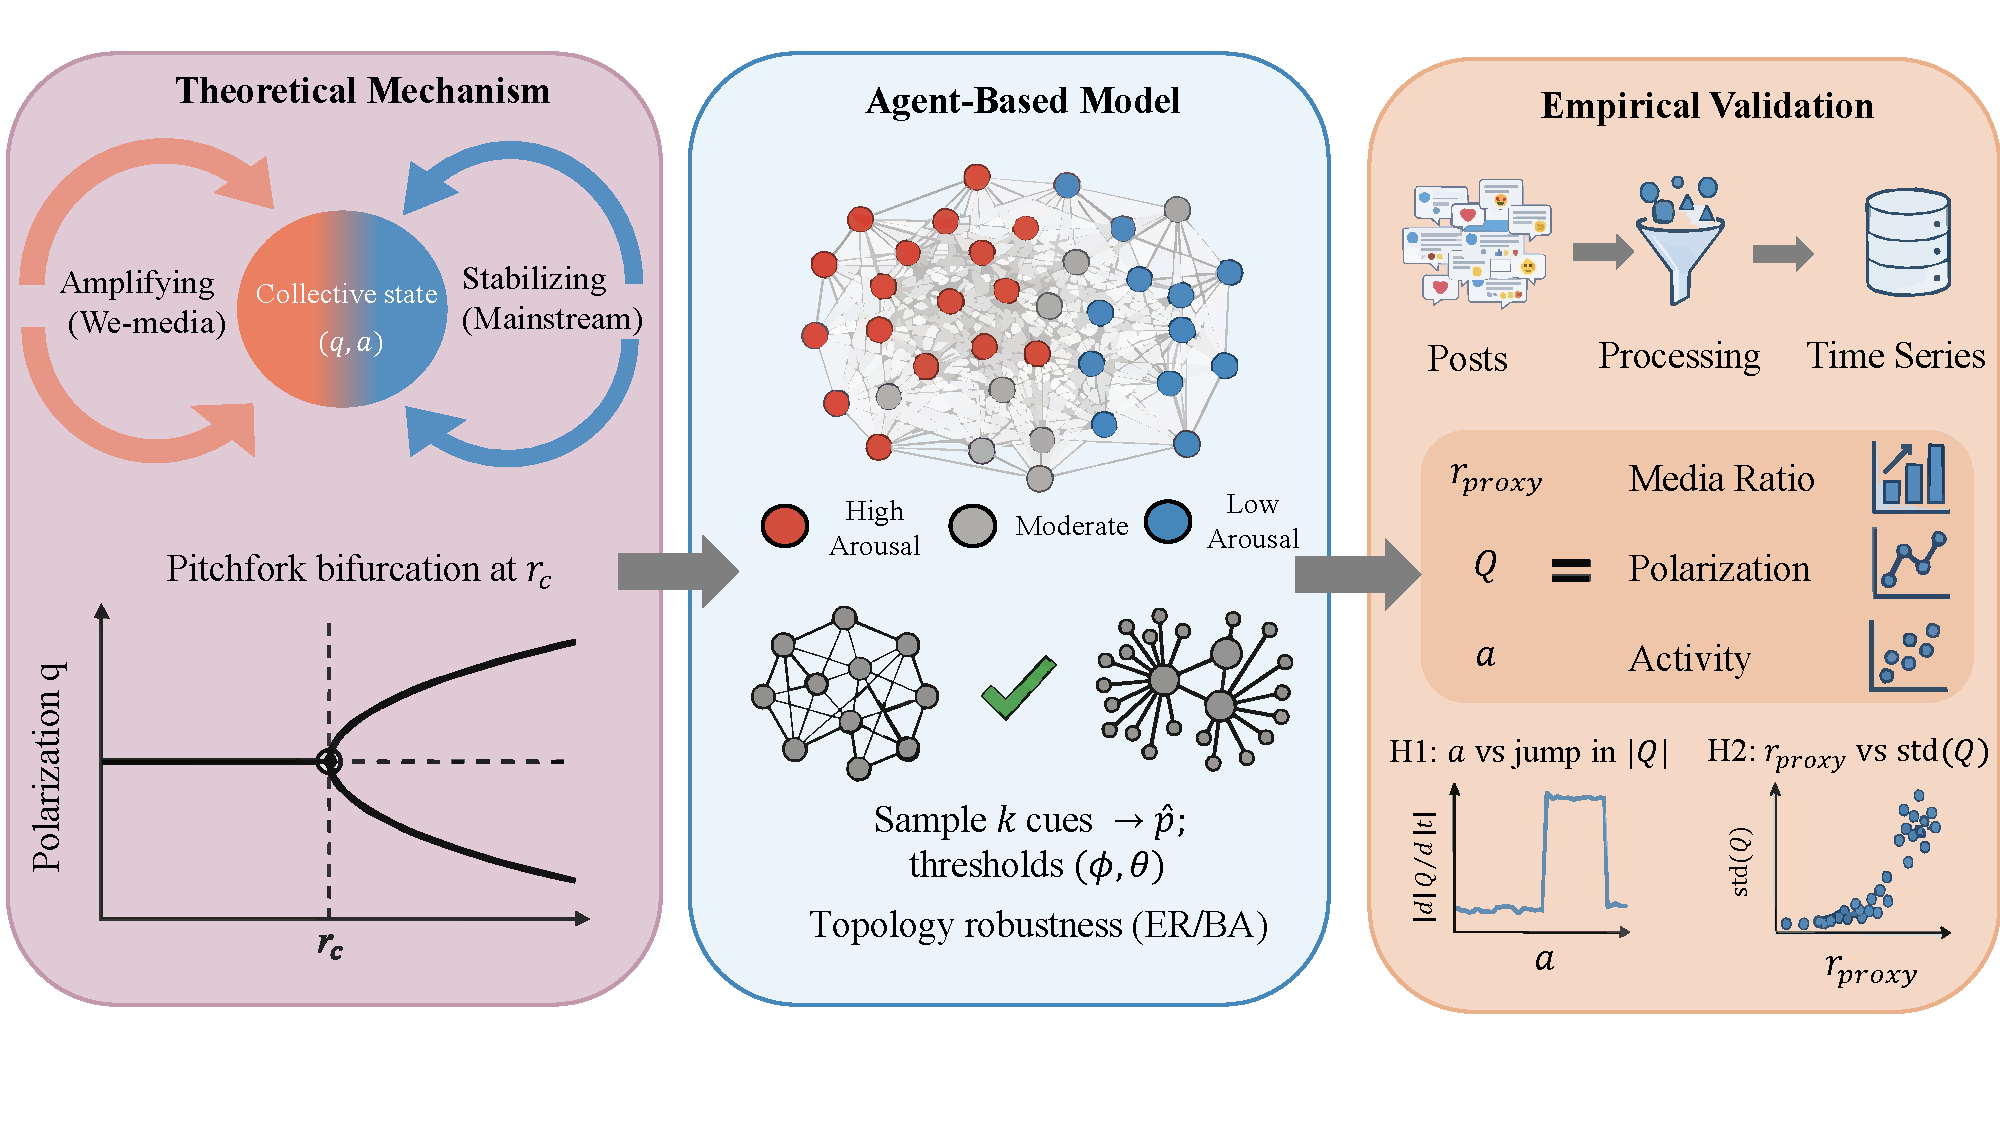
\includegraphics[width=0.95\linewidth]{fig0_framework.pdf}
  \vspace{0.4em}
  \small Theory (bifurcation) $\rightarrow$ Parameter landscape $\rightarrow$ Network robustness $\rightarrow$ Dynamical precursors (CSD) $\rightarrow$ Empirical signatures
\end{frame}

\begin{frame}{Mixed-feedback mechanism (two competing channels)}
  \begin{columns}[T,onlytextwidth]
    \begin{column}{0.55\textwidth}
      \begin{itemize}
        \item Two channels shape perceived risk: a stabilizing mainstream channel and an amplifying user-generated channel.
        \item A single control parameter $r\in[0,1]$ shifts channel balance.
        \item Key question: when does the neutral state lose stability, and what signatures precede it?
      \end{itemize}
    \end{column}
    \begin{column}{0.45\textwidth}
      \centering
      \includesvg[width=\linewidth]{csdag}
    \end{column}
  \end{columns}
\end{frame}

\begin{frame}{Direction vs intensity (state variables) + mean-field bifurcation}
  \begin{columns}[T,onlytextwidth]
    \begin{column}{0.46\textwidth}
      \begin{block}{Macroscopic variables}
        \vspace{-0.3em}
        \[
          q=\rho_H-\rho_L \quad \text{(direction)},\qquad
          a=\rho_H+\rho_L=1-\rho_M \quad \text{(intensity)}
        \]
        \vspace{-0.6em}
      \end{block}
      \begin{itemize}
        \item $a$ tracks depletion of the moderate buffer $\rho_M$.
        \item Mean-field analysis yields an analytic critical point $r_c$.
      \end{itemize}
    \end{column}
    \begin{column}{0.54\textwidth}
      \centering
      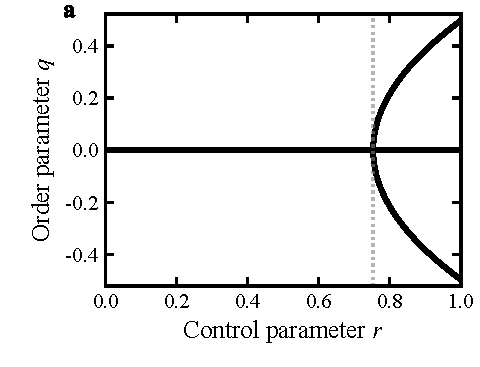
\includegraphics[width=\linewidth]{fig1a_bifurcation.pdf}
    \end{column}
  \end{columns}
\end{frame}

\begin{frame}{Bistability as loss of resilience}
  \begin{columns}[T,onlytextwidth]
    \begin{column}{0.45\textwidth}
      \begin{itemize}
        \item As stabilizing feedback is down-weighted, the effective potential changes from a single well to a double well.
        \item Bistability provides a mechanistic picture of ``emotional bubbles'' as a loss of resilience.
      \end{itemize}
    \end{column}
    \begin{column}{0.55\textwidth}
      \centering
      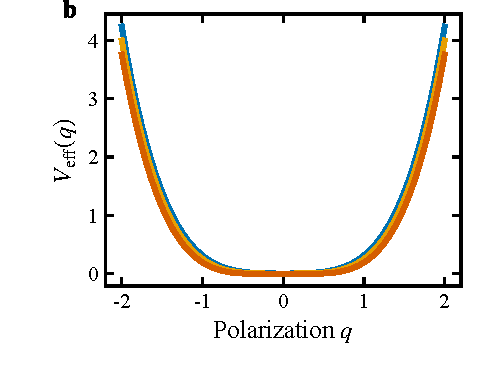
\includegraphics[width=\linewidth]{fig1b_potential.pdf}
    \end{column}
  \end{columns}
\end{frame}

\begin{frame}{Symmetric vs asymmetric regimes: direction--intensity entanglement}
  \begin{itemize}
    \item Symmetric validation regime: sharp tipping in $q$, activity rises mainly near $r_c$.
    \item Activity-coupled asymmetry: direction and intensity rise together for $r<r_c$, producing a broader crossover.
  \end{itemize}
  \centering
  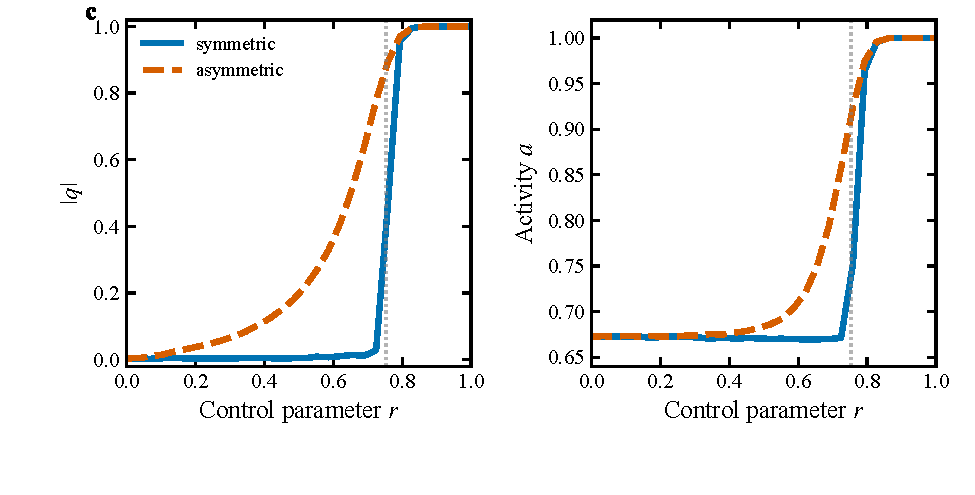
\includegraphics[width=0.95\linewidth]{fig1c_sym_asym_qa.pdf}
\end{frame}

\begin{frame}{Parameter landscape: where is the system fragile?}
  \begin{itemize}
    \item The critical boundary $r_c$ depends on psychological thresholds and response sensitivity.
    \item A transition exists only when the collective sensitivity is sufficiently high.
  \end{itemize}
  \centering
  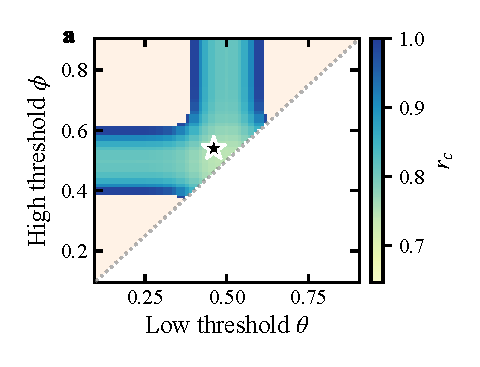
\includegraphics[height=0.56\textheight,keepaspectratio]{fig4a_chi_rc_landscape.pdf}
\end{frame}

\begin{frame}{Structural levers: information density and media ecology}
  \begin{columns}[T,onlytextwidth]
    \begin{column}{0.50\textwidth}
      \centering
      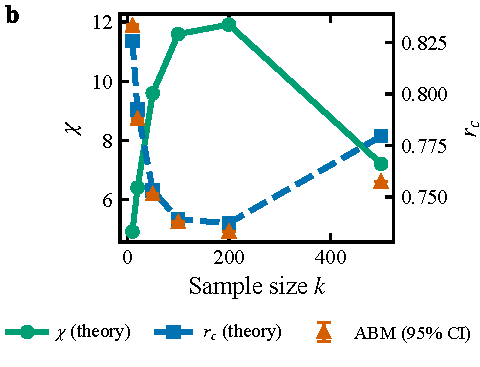
\includegraphics[width=\linewidth]{fig4b_k_effect.pdf}
      \vspace{0.2em}
      \small Information density reshapes sensitivity and shifts $r_c$.
    \end{column}
    \begin{column}{0.50\textwidth}
      \centering
      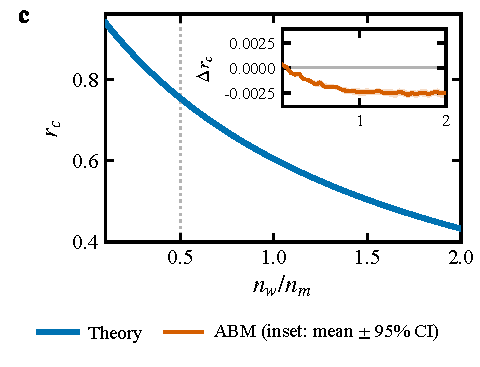
\includegraphics[width=\linewidth]{fig4c_media_ratio.pdf}
      \vspace{0.2em}
      \small Greater user-generated dominance lowers $r_c$ (more fragile).
    \end{column}
  \end{columns}
\end{frame}

\begin{frame}{Structural levers: local coupling}
  \begin{itemize}
    \item Local reinforcement can shift the macroscopic boundary and bias branch selection.
    \item Interpretable as network-mediated amplification beyond the global environment.
    \item ABM max-slope estimates of $r_c(\beta)$ shift downward as local coupling increases, consistent with network-mediated amplification.
  \end{itemize}
  \centering
  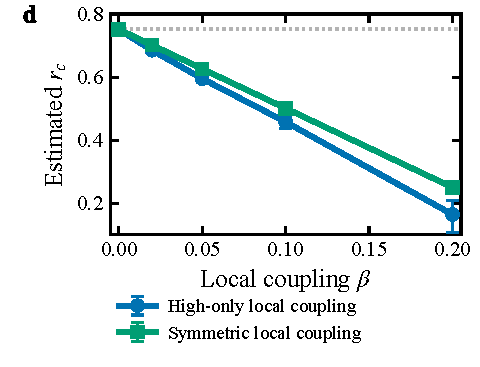
\includegraphics[height=0.54\textheight,keepaspectratio]{fig4d_beta_effect.pdf}
\end{frame}

\begin{frame}{Network validation: bifurcation persists beyond mean-field}
  \begin{columns}[T,onlytextwidth]
    \begin{column}{0.50\textwidth}
      \centering
      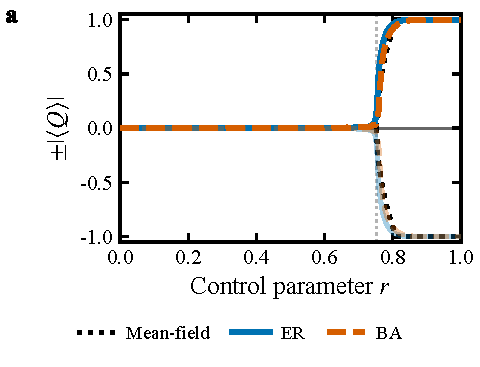
\includegraphics[width=\linewidth]{fig2a_network_validation.pdf}
      \vspace{0.2em}
      \small Symmetry implies branch selection; use $|Q|$ or sign alignment.
    \end{column}
    \begin{column}{0.50\textwidth}
      \centering
      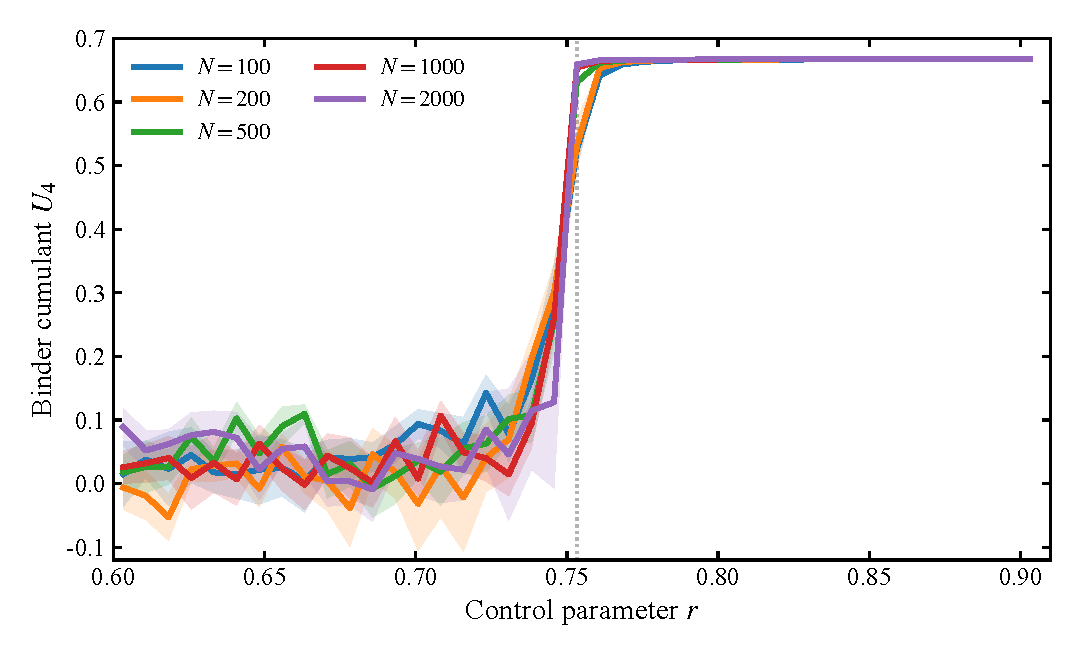
\includegraphics[width=\linewidth]{fig2b_binder_u4.pdf}
      \vspace{0.2em}
      \small Binder cumulant crossings locate $r_c$ robustly at finite size.
    \end{column}
  \end{columns}
\end{frame}

\begin{frame}{Network validation: activity dynamics}
  \begin{itemize}
    \item Under symmetry, activity rises mainly near $r_c$.
    \item Under activity-coupled asymmetry, activity increases earlier, consistent with direction--intensity coupling.
  \end{itemize}
  \centering
  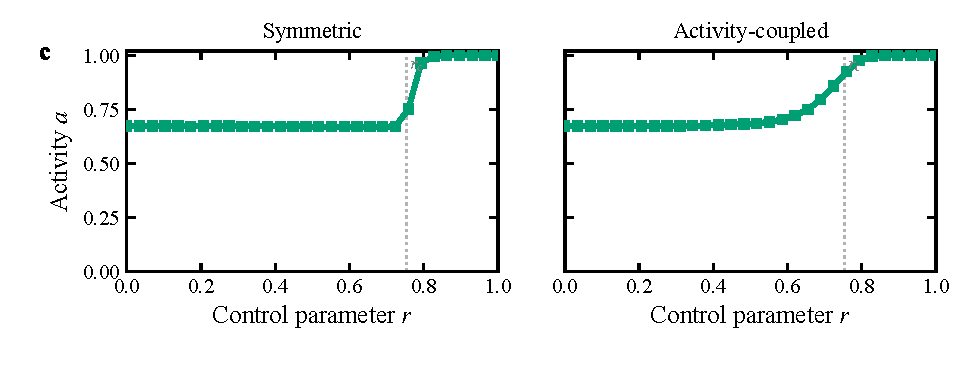
\includegraphics[width=0.92\linewidth]{fig2c_activity.pdf}
\end{frame}

\begin{frame}{Critical slowing down: a leading indicator}
  \begin{columns}[T,onlytextwidth]
    \begin{column}{0.50\textwidth}
      \centering
      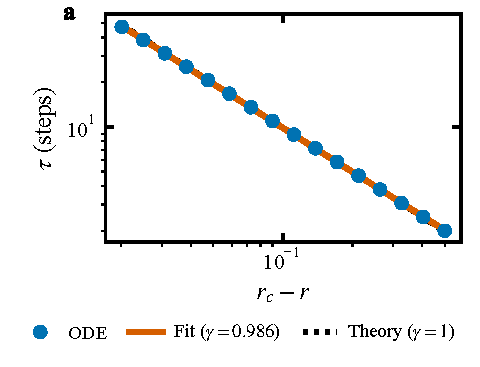
\includegraphics[width=\linewidth]{fig3a_csd_scaling.pdf}
      \vspace{0.2em}
      \small Mean-field: $\tau \propto (r_c-r)^{-1}$ for $r<r_c$.
    \end{column}
    \begin{column}{0.50\textwidth}
      \centering
      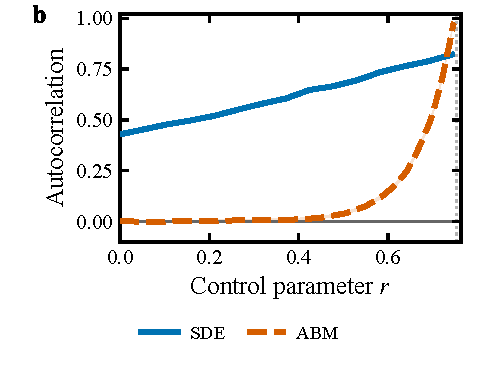
\includegraphics[width=\linewidth]{fig3b_csd_sde_vs_abm.pdf}
      \vspace{0.2em}
      \small SDE and ABM: rising short-lag autocorrelation as $r\to r_c$.
    \end{column}
  \end{columns}
\end{frame}

\begin{frame}{Trajectory intuition}
  \begin{itemize}
    \item Far from criticality: fast recovery within a few sweeps.
    \item Near criticality: prolonged fluctuations and slow recovery.
  \end{itemize}
  \centering
  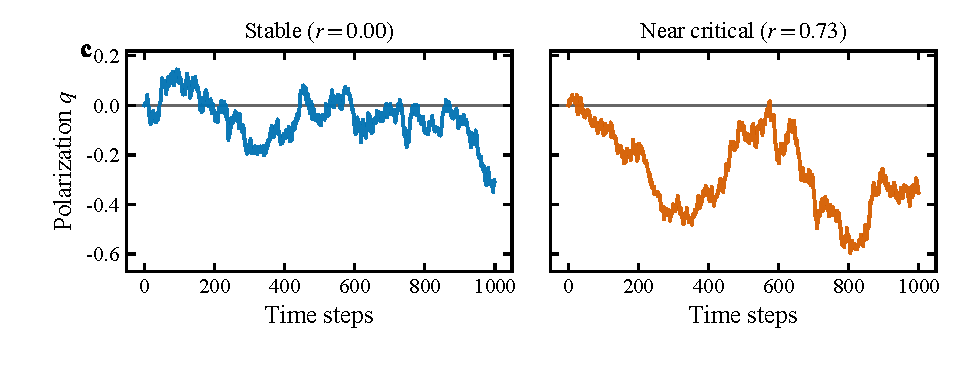
\includegraphics[width=0.92\linewidth]{fig3c_csd_timeseries.pdf}
\end{frame}

\begin{frame}{From model to data: empirical proxies (high level)}
  \small
  \begin{center}
    \begin{tabular}{@{}ll@{}}
      \toprule
      \textbf{Model variable} & \textbf{Empirical proxy (segment-level)} \\
      \midrule
      Direction $q$ & $Q = X_H - X_L$ \\
      Intensity $a$ & $a = X_H + X_L = 1 - X_M$ \\
      Channel balance & $r_{\mathrm{proxy}} = \dfrac{n_{\mathrm{wemedia}}}{n_{\mathrm{wemedia}}+n_{\mathrm{mainstream}}+n_{\mathrm{government}}}$ \\
      Jump intensity & $\text{jump}_{q95}$ (upper-tail change in $|Q|$) \\
      Volatility & $\mathrm{std}(Q)$ \\
      \bottomrule
    \end{tabular}
  \end{center}
  \vspace{0.4em}
  \begin{itemize}
    \item Weekly segments balance temporal resolution and coverage.
    \item H2 uses 12-hour aggregation for more stable within-segment estimation under missingness.
  \end{itemize}
\end{frame}

\begin{frame}{Empirical signatures (H1/H2)}
  \begin{columns}[T,onlytextwidth]
    \begin{column}{0.50\textwidth}
      \centering
      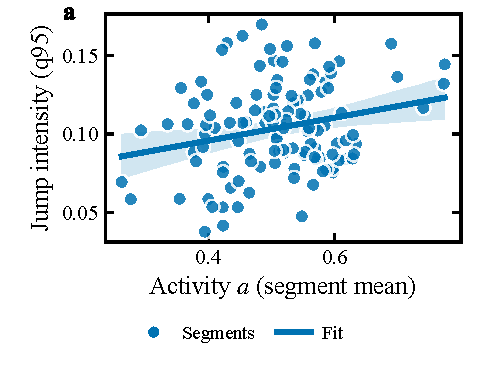
\includegraphics[width=\linewidth]{fig5a_activity_jump.pdf}
      \vspace{0.2em}
      \small H1: higher activity is associated with larger jump intensity.
    \end{column}
    \begin{column}{0.50\textwidth}
      \centering
      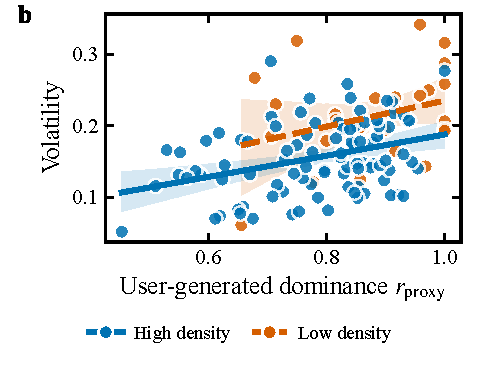
\includegraphics[width=\linewidth]{fig5b_media_volatility_density.pdf}
      \vspace{0.2em}
      \small H2: under sufficient temporal sampling, higher $r_{\mathrm{proxy}}$ is associated with higher volatility.
    \end{column}
  \end{columns}
  \vspace{0.4em}
  \small
  \begin{itemize}
    \item H1 (pooled, 4H): Pearson $r=0.241$, $p=0.00798$.
    \item H2 (high-density, 12H): Pearson $r=0.429$, $p=6.03\times 10^{-7}$; density-controlled partial $r=0.386$, $p=8.79\times 10^{-6}$.
  \end{itemize}
\end{frame}

\begin{frame}{Takeaways \& call-to-action}
  \begin{block}{Core contributions (what is new)}
    \begin{itemize}
      \item Reframes polarization as endogenous structural instability driven by channel balance, moving beyond external-shock explanations.
      \item A minimal mixed-feedback mechanism with a single control parameter linking media ecology to resilience.
      \item Direction--intensity decomposition connecting transitions to observable precursors (activity).
      \item Multi-level evidence chain: theory $\rightarrow$ parameter landscape $\rightarrow$ network robustness $\rightarrow$ dynamical precursors $\rightarrow$ empirical signatures.
    \end{itemize}
  \end{block}
  \begin{block}{Decisions / help needed}
    \begin{itemize}
      \item Results structure: keep ``parameter landscape $\rightarrow$ network robustness $\rightarrow$ CSD'' order?
      \item Empirical H2: keep 12-hour aggregation as primary (4H shown as density-sensitive diagnostic)?
      \item Submission strategy: prioritize Nature Human Behaviour vs Nature Communications?
    \end{itemize}
  \end{block}
\end{frame}

\appendix
\section*{Backup}

\begin{frame}{Backup: H2 density diagnostics (4H vs 12H)}
  \begin{block}{Key point}
    \small 12H aggregation stabilizes within-segment estimates under missingness; 4H diagnostics are more sensitive to sparse coverage.
  \end{block}
  \begin{columns}[T,onlytextwidth]
    \begin{column}{0.50\textwidth}
      \centering
      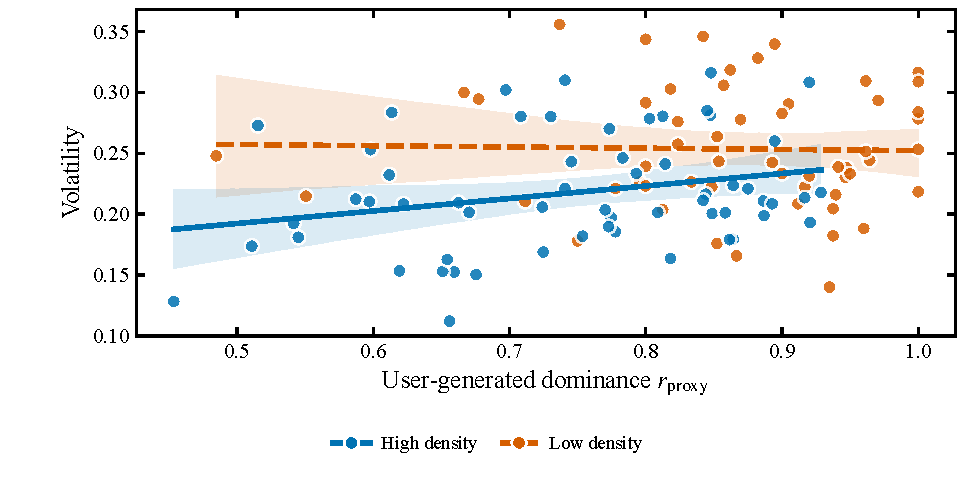
\includegraphics[width=\linewidth]{s5_h2_density_4h.pdf}\par
      \vspace{0.2em}
      \scriptsize 4H aggregation
    \end{column}
    \begin{column}{0.50\textwidth}
      \centering
      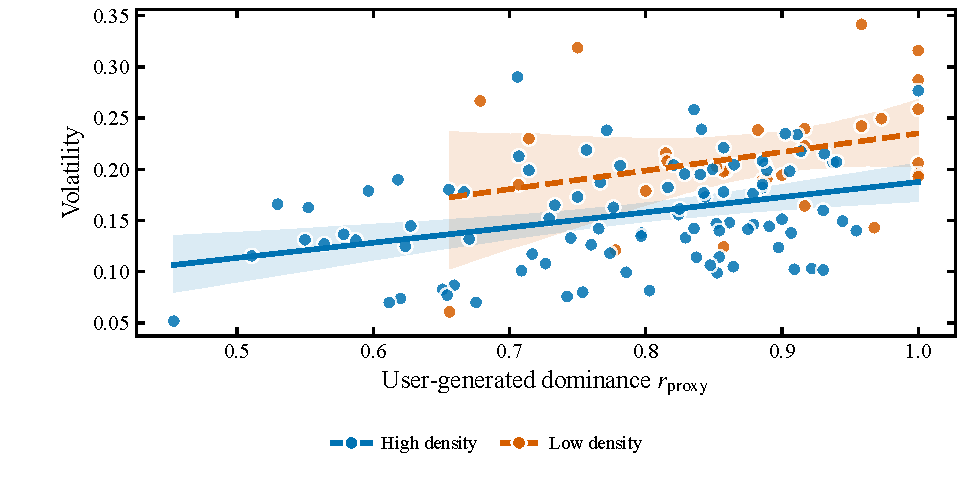
\includegraphics[width=\linewidth]{s5_h2_density_12h.pdf}\par
      \vspace{0.2em}
      \scriptsize 12H aggregation
    \end{column}
  \end{columns}
\end{frame}

\begin{frame}{Backup: activity relaxes faster than polarization under asymmetry}
  \small Asymmetric simulations show $\tau_a/\tau_q\approx 0.70$, supporting direction--intensity coupling.
  \centering
  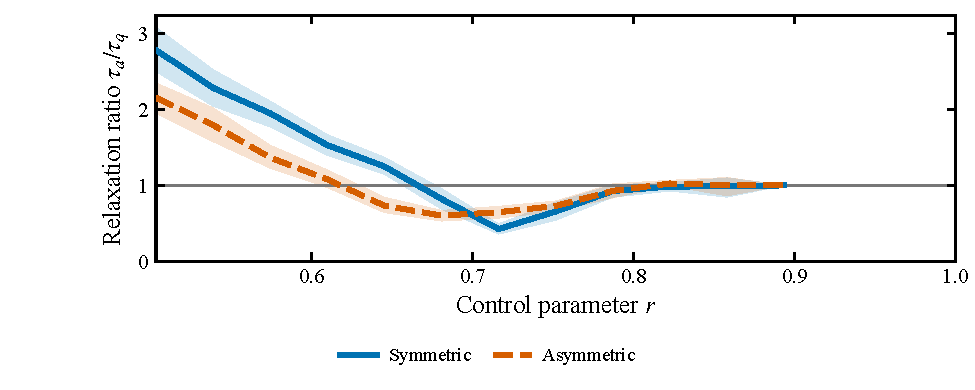
\includegraphics[height=0.70\textheight,keepaspectratio]{s2_tau_ratio.pdf}
\end{frame}

\begin{frame}{Backup: empirical test summary}
  \small
  \begin{center}
    \begin{tabular}{@{}lccc@{}}
      \toprule
      \textbf{Test} & \textbf{Dataset} & \textbf{Aggregation} & \textbf{Estimate} \\
      \midrule
      Activity $\rightarrow$ Jump intensity & Pooled & 4H & $r=0.241$ ($p=0.00798$) \\
      $r_{\mathrm{proxy}}\rightarrow$ Volatility & High-density & 12H & $r=0.429$ ($p=6.03\times 10^{-7}$) \\
      \bottomrule
    \end{tabular}
  \end{center}
  \vspace{0.4em}
  \begin{itemize}
    \item H2 density-controlled partial correlation (12H): $r=0.386$ ($p=8.79\times 10^{-6}$).
  \end{itemize}
\end{frame}

\begin{frame}{Backup: LLM annotation (summary)}
  \begin{itemize}
    \item Model: \texttt{Qwen/Qwen3-8B} served via vLLM (OpenAI-compatible API).
    \item Structured prompt + fixed JSON schema; temperature $=0.1$, max\_tokens $=512$.
    \item Human validation subset ($n=5{,}000$): arousal accuracy 85\% ($\kappa=0.79$), risk accuracy 87\% ($\kappa=0.82$).
  \end{itemize}
\end{frame}

\end{document}
